\begin{savequote}[6cm]
<< Is this thing on? I don't think this thing is on. Hello! [...] Confangled modern doohickeys. >>
\qauthor{Grany Smith}
\end{savequote}

\chapter{Astronef : De l'expression à l'exécution}\label{chap:contrib:astronef}
\chaptertoc

Astral est une algèbre permettant des requêtes continues sans ambiguïtés sémantiques. Les concepts développés au chapitre~\ref{chap:contrib:astral} ne sont pas attachés à un mode d'exécution ou à une implémentation particulière. Dans ce chapitre, nous présentons l'intergiciel \textit{Astronef}\footnote{Astral Optimization and Execution Framework} permettant l'exécution de requêtes continues Astral. Dans cette mise en œuvre, nous focalisons notre attention sur trois points en particulier :
\begin{itemize}
	\item[\textbf{Conformité à Astral}] : Nous avons développé un modèle expressif et libre de toute ambiguïté. Il est important que les composants développés dans cette mise en œuvre puissent exprimer les sémantiques que chacun est capable d'exécuter.
	\item[\textbf{Extensibilité}] : L'utilisateur doit pouvoir adapter l'intergiciel à son utilisation. Ainsi, il doit pouvoir ajouter ou reconfigurer des composants à la volée.
	\item[\textbf{Optimisation}] : L'intergiciel doit être capable de fournir un plan d'exécution efficace pour une requête donnée.
\end{itemize}

La section~\ref{sec:contrib:astronef:architecture} présente l'architecture générale d'Astronef. La section~\ref{sec:contrib:astronef:preparation} présente notre approche à base de règle pour construire un plan de requête. La section~\ref{sec:contrib:astronef:logique} présente la première partie de l'optimisation du plan : l'optimisation logique, permettant de réécrire une requête de manière plus efficace. Puis nous détaillons en section~\ref{sec:contrib:astronef:physique} la seconde partie de l'optimisation : l'optimisation physique permettant de sélectionner les meilleurs composants pour exécuter le plan de requête. Enfin, nous analysons en section~\ref{sec:contrib:astronef:integration} les impacts de l'intégration d'un nouveau composant à l'architecture. Nous concluons ce chapitre en section~\ref{sec:contrib:astronef:conclusion}.

\lstset{language=PrologAstral}
\section{De l'algèbre aux composants}\label{sec:contrib:astronef:architecture}
Dans cette section, nous détaillons les éléments d'architectures que nous avons mis en œuvre pour permettre à une requête Astral d'être instanciée en un processus de traitement. Nous abordons premièrement les principes architecturaux utilisés. Ensuite, nous détaillons les différents composants utilisés dans Astronef. Enfin, nous présentons notre méthode extensible de construction de plan par l'utilisation d'un système de règles.
\subsection{Architecture}
Avant de détailler l'architecture de notre système de traitement de requêtes continues, nous allons d'abord présenter le paradigme architectural dans lequel nous allons mettre en œuvre Astronef. Nous présentons premièrement et brièvement les architectures à services. Puis, nous détaillons les principes des architectures à composants orientés services que nous utilisons par la suite.
\subsubsection{Architecture à service}
Les architectures à services permettent aux applications d'être assemblés sous forme de blocs réutilisables étant des \textit{services}. Un \textit{service} est définit par une spécification (ou \textit{description}, ou \textit{contrat}), qui décrit sa syntaxe, son comportement, sa sémantique ainsi que sa dépendance aux autres services. Dans les architectures à service, les services interagissent via un patron récurrent d'interaction (fig~\ref{fig:contrib:astronef:services}). 
\begin{figure}[ht]
    \centering
    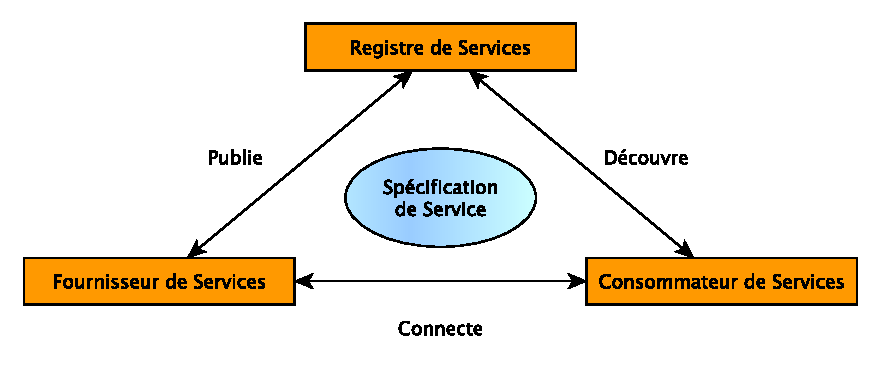
\includegraphics[width=0.7\textwidth]{contrib-astronef-services}
    \caption{Patron d'interaction de service}\label{fig:contrib:astronef:services}
\end{figure}
Un fournisseur de service va publier sa spécification à un registre. Un consommateur de service découvre le service fournit par une requête sur le registre. Enfin, le consommateur et le fournisseur se connectent. Le point clé de cette architecture étant que cette résolution est faite au \textit{runtime}.

\subsubsection{Architecture à composants orientés services}
Le modèle d'architecture à composants orientés services~\cite{Cervantes:servicecomponent} permet la mise en œuvre d'applications à base de services dans le paradigme de la programmation par composants. Le principe étant de séparer les mécanismes des architectures à services du code implémentant le comportement du service fournit. Ainsi, voici les principes d'un tel modèle :
\begin{itemize}
    \item Un service est une fonctionnalité fournie.
    \item Un service est caractérisé par sa spécification.
    \item Les composants implémentent des spécifications de services, qui peuvent eux-mêmes dépendre, du fait de leurs implémentations, d'autres services.
    \item Les patrons d'interactions de services sont utilisés pour résoudre les dépendances de services au \textit{runtime}.
    \item Les compositions sont décrites en terme de spécifications de services.
    \item Tout composant peut se substituer par un autre si les spécifications de services sont identiques.
\end{itemize}
Nous mêlons donc dans un même modèle, les idées de composants et de services. De plus, en s'inspirant des modèles récents tels que Fractal~\cite{Bruneton:fractal}, chaque composant possède un ensemble de propriétés (ou attributs) configurables. Nous obtenons aussi le pouvoir d'instancier (grâce aux fabriques) des composants à partir de configurations.

\begin{figure}[ht]
    \centering
    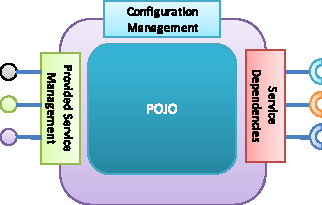
\includegraphics[width=0.5\textwidth]{contrib-astronef-ipojo}
    \caption{Un composant iPojo}\label{fig:contrib:astronef:ipojo}
\end{figure}
La figure~\ref{fig:contrib:astronef:ipojo} représente un composant dans l'implémentation \textit{iPojo}~\cite{Escoffier:ipojo}. Le principe étant que le code du composant (le \textit{POJO}, \textit{Plain Old Java Object}) est embarqué dans un conténaire auxquels seront accrochés des gestionnaires. Les trois couramment utilisés sont les gestionnaires de dépendances, de production de service, et de configuration. Ainsi, un composant pourra s'exposer sur un registre, tout en dépendant d'autres services et en supportant le fait d'être configurable.

\subsection{Les différents composants et services}
L'architecture d'Astronef est entièrement dirigé par ces approches. De multiples composants sont ainsi créés et instantiables, pour former une requête. Afin de pouvoir exécuter les requêtes, nous définissons trois services centraux :
\begin{itemize}
	\item[\textbf{Les \textit{EventProcessor}}] : Ces services ont deux primitives, l'une exécute une tâche quelconque, l'autre indique les autres \textit{EventProcessors} dont il dépend.
	\item[\textbf{Le \textit{Scheduler}}] : Ce service permet la planification. Ses primitives permettent aux différents \textit{EventProcessor} d'exprimer leur volonté de s'exécuter. Ce service devra mettre en ordre ces demandes en fonction des dépendances exprimés.
	\item[\textbf{Le \textit{QueryRuntime}}] : Ce service permet d'exécuter une requête. Il est lié à un \textit{Scheduler}, et utilise la primitive \textit{next} de celui-ci pour connaître la prochaine tâche qu'il faudra exécuter.
\end{itemize}

Nous adoptons ainsi l'approche émise par~\cite{Carney:scheduling} pour gérer l'ordonnancement des événements. Maintenant que nous avons vu les différents services nécessaire à l'exécution. Nous avons plusieurs types de composants que nous pourrons instantier :
\begin{itemize}
	\item[\textbf{Les entités}] : Fournissent les services nécessaires pour manipuler un flux ou une relation. Ces entités servent de résultats intermédiaires (ou de tampons). De plus, ils permettent un service de notification. En cas de changement, les \textit{EventProcessor} abonnés seront notifiés. Ainsi, ces composants nécessitent un \textit{Scheduler} pour demander l'exécution de leurs abonnés.
	\item[\textbf{Les sources}] : Une source nécessite une entité en lecture, dont elle manipulera le contenu pour la remplir. Ce composant pourra nécessiter le \textit{Scheduler} pour, entre autres, notifier la fin de son envoi et donc la fin de la requête.
	\item[\textbf{Les opérateurs}] : Nécessitent $n$ entités en lecture, et une autre particulière en écriture. Ce composant doit fournir le service \textit{EventProcessor}. Les implémentations des opérateurs bloquants pourront faire appel au \textit{Scheduler} pour planifier des exécutions ponctuelles.
	\item[\textbf{Les puits}] : Nécessitent une entité en lecture. Ce composant fournit le service \textit{EventProcessor} et doit être non-bloquant (donc seulement s'abonner à son entité en lecture).
\end{itemize}

Ainsi pour créer une requête : l'utilisateur doit fournir un ou plusieurs composants sources et un composant puit. Par la suite, il demande à Astronef de lui instantier ses sources et son puit en configurant les composants selon sa volonté. Enfin, il spécifie l'expression algébrique liant les sources au puit.

\subsubsection{De l'importance de la réutilisation}
Le fait d'abstraire l'architecture d'\textit{Astronef} permet une grande flexibilité architecturale. Tout d'abord, pour chaque composant, le fait de pouvoir le configurer tout en gérant son cycle de vie permet de réutiliser le même module pour plusieurs usages. Par exemple, supposons l'existance d'une source capable de récupérer une information périodiquement sur un protocole donné. Cette source pourra être utilisé pour plusieurs requêtes sous différentes instances en ayant plusieurs configurations.

Mais cette abstraction sous forme de services permet surtout la substitution. En effet, nous pouvons remplacer n'importe quel composant du moment qu'il supporte le même service. Nous utilisons ce principe pour sélectionner les meilleurs composants pour remplir le plus efficacement leurs rôles. De plus, l'utilisateur peut apporter ses propres implémentations pour étendre les capacités de l'intergiciel.

\subsection{Construction du plan par règles}
Nous définissons un plan de requête comme un ensemble de composants déployés pour répondre à la requête de l'utilisateur. Nous souhaitons avant tout que l'utilisateur n'ai pas à intervenir lors de cette construction. De son point de vue, il ne doit écrire que l'expression algébrique de sa requête et il doit être garanti d'une mise en œuvre efficace.

Pour atteindre ce but, nous avons choisi de mettre en place un moteur de règle. Le principe étant que nous partons de l'expression algébrique, puis nous itérons suivant plusieurs schéma d'inférences jusqu'à obtenir un plan de requête. Nous remarquons plusieurs avantage à une telle approche :
\begin{itemize}
	\item Intégration naturelle des connaissances. L'algèbre est pleine de propriété et de théorèmes. Il est nécessaire de pouvoir les exprimer dans un langage déclaratif pour les exploiter et pour en rajouter le plus possible.
	\item Expression de la sémantique des composants par l'algèbre. Comme il est nécessaire d'associer des composants logiciels à la sémantique d'Astral, il est nécessaire de spécifier à quelle opération chaque composant (et chaque paramètre de configuration) répond. Cela permet une clarification des sémantiques d'exécution.
	\item Extensibilité très forte. En considérant que l'ajout de nouveaux composants peut se faire via l'ajout de nouvelles règles, il devient aisé d'étendre le système pour permettre des opérateurs, ou des optimisations qui n'étaient pas prévues.
\end{itemize}

Afin de mettre en œuvre cet ensemble de règle pour obtenir un plan de requête efficace, nous faisons une analogie avec les systèmes de gestions de base de données. Comme présenté dans la section~\ref{sec:rw:sgfd:optim}, l'optimisation est découpé en deux parties : l'optimisation logique, et l'optimisation physique. Nous réutiliserons cette approche qui a fait ses preuves au fur et à mesure des années. Nous restructurerons donc la structure de l'expression algébrique dans la section~\ref{sec:contrib:astronef:logique} pour qu'elle soit plus optimisé. Ensuite, nous sélectionnerons les meilleurs composants et les meilleures configurations pour mettre en œuvre cette nouvelle expression, dans la section~\ref{sec:contrib:astronef:physique}.

Nous utilisons un moteur capable d'exécuter du Prolog~\footnote{En réalité, le langage utilisé (PROVA~\cite{Kozlenkov:prova}) est un dérivé de Prolog mieux adapté à l'intégration avec Java. Mais le principe reste tout à fait similaire.}, langage de programmation logique, pour appliquer nos règles. Avant de détailler l'ensemble de ces règles, nous présentons d'abord la structure d'une expression. Toute expression étant structuré sous forme d'arbre, il est possible de représenter une requête avec des nœuds de la forme\footnote{L'utilisation d'objets de propriétés fait partie du langage PROVA, mais cela reste formalisable en Prolog standard avec une liste d'éléments [clé,valeur].} :
\begin{center} [$\underbrace{A}_{\textrm{Nature du nœud}}$, $\underbrace{B}_{\textrm{Ensemble de propriétés}}$, $\underbrace{C}_{\textrm{Liste de nœuds fils}}$] \end{center}
\begin{example}
	Soit $R$ une source déclaré dans le système, nous souhaitons exécuter la requête $\sigma_{id=1} R$. Alors l'expression de cette requête est la suivante :
	\begin{lstlisting}
[sigma,	{"condition":"id=1"}, [
	[source, {id:"R"}, []]
]]
	\end{lstlisting}
\end{example}
Nous remarquons que cette syntaxe est très similaire au \textit{XML}, c'est pour cela que ce langage est celui utilisé en pratique pour spécifier des requêtes dans le prototype. Il est ensuite traduit en expression utilisable en Prolog. L'ensemble des nœuds possibles corresponds aux différents opérateurs de l'algèbre. Nous ne détaillerons pas ceci dans ce manuscrit. Le lecteur pourra consulter le manuel sur la page web suivante \url{http://code.google.com/p/astral/wiki/XMLSyntax} pour trouver les expressions exactes supportées.
\section{De l'algèbre aux composants}\label{sec:contrib:astronef:preparation}
À tout composant est attachée une fabrique permettant de créer les instances. Pour construire une requête, l'utilisateur d'Astronef peut faire appel à chaque fabrique pour instancier chaque source, opérateur, entité, et puits. Une fois les composants construits et liés entre eux, il peut demander au moteur de créer un service \textit{QueryRuntime} pour exécuter la requête. Toutefois, nous souhaitons pouvoir exploiter les connaissances d'Astral pour aider à la construction de ce plan d'exécution. Ainsi, l'utilisateur n'a pas à intervenir lors de la construction de la requête.

En effet, de son point de vue, il ne doit écrire que l'expression algébrique de sa requête et il doit être garanti d'une mise en œuvre efficace. Cette section détaille notre approche. Tout d'abord, nous détaillons l'idée de la construction du plan d'exécution par règles. Ensuite, nous présentons les choix technologiques mis en œuvre. Enfin, nous voyons comment préparer la requête à l'optimisation que nous détaillons dans les sections suivantes.

\subsection{Approche de la construction de requêtes par inférence}
Pour atteindre une construction \textit{automatique}, nous avons choisi de mettre en place une approche à base de règles. En partant de l'expression algébrique, nous itérons suivant plusieurs règles d'inférence jusqu'à l'obtention d'un plan de requête. Nous remarquons plusieurs avantages à une telle approche :
\begin{itemize}
	\item Intégration naturelle des connaissances. Les propriétés de l'algèbre peuvent s'exprimer dans un langage déclaratif pour les exploiter.
	\item Expression de la sémantique des composants par l'algèbre. Comme il est nécessaire d'associer la sémantique d'Astral aux composants logiciels, il est nécessaire de spécifier à quelle opération chaque composant (et chaque paramètre de configuration) répond. Cela permet une clarification des sémantiques d'exécution.
	\item Extensibilité très forte. En considérant que l'ajout de nouveaux composants peut se faire via l'ajout de nouvelles règles, il devient aisé d'étendre le système pour permettre des opérateurs, ou des optimisations qui n'étaient pas prévues.
\end{itemize}

\subsubsection{Optimisation par heuristiques}
Afin de mettre en œuvre cet ensemble de règles pour obtenir un plan de requête efficace, nous introduisons une optimisation logique et physique à l'image des optimisations des SGBD. Nous restructurons la structure de l'expression algébrique dans la section~\ref{sec:contrib:astronef:logique} pour qu'elle soit plus optimisée. Ensuite, nous sélectionnons les meilleurs composants et les meilleures configurations pour mettre en œuvre cette nouvelle expression, dans la section~\ref{sec:contrib:astronef:physique}.

Toutefois, dans notre contexte, nous ne pouvons pas appliquer directement certaines optimisations des SGBDs. Contrairement aux règles habituelles, nous ne réordonnons pas les jointures du fait du théorème~\ref{thm:asymetrie}. De plus, la notion d'entrée-sortie est réduite à une notion de résultats intermédiaires, même au niveau des sources (rendant l'utilisation des index moins pertinents que sur disque). En effet, la performance se mesure généralement en débit supporté et les débits de sources sont a priori inconnus. Au total, un gain de performance est mesuré sur un gain de consommation processeur et, à moindre mesure, sur une consommation mémoire contrôlée (ou bornée).

De plus, Astral possède plus d'opérateurs et de restrictions que l'algèbre relationnelle ce qui rend l'espace de recherche plus large. Ainsi, nous développons plusieurs heuristiques nous permettant de faire les différentes réécritures par applications de règles.

\begin{figure}[ht]
	\centering
	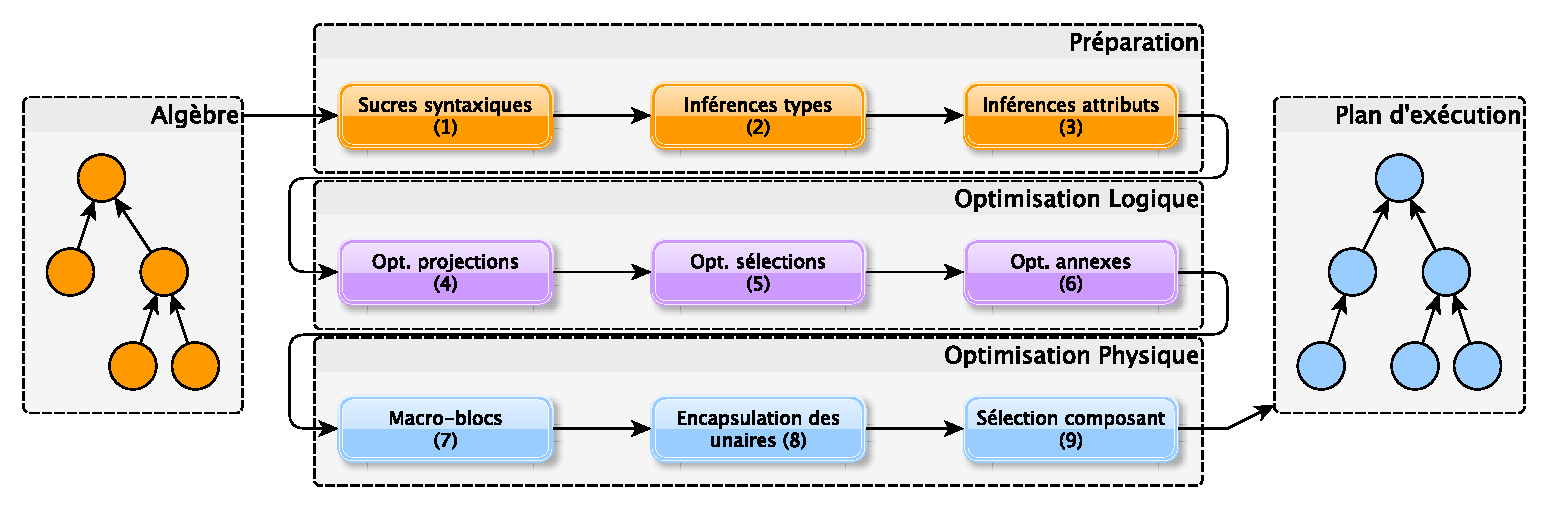
\includegraphics[width=0.9\textwidth]{contrib-astronef-optimisation}
	\caption{Processus d'optimisation d'une requête algébrique dans Astronef}\label{fig:contrib:astronef:optimisation}
\end{figure}
La figure~\ref{fig:contrib:astronef:optimisation} représente le processus total d'optimisation d'une requête algébrique. Nous pouvons clairement distinguer trois parties, la phase de préparation, puis l'optimisation logique et enfin physique. Chaque sous-tâche est détaillée dans la suite de ce chapitre.

\subsection{Expression d'une requête}
Nous utilisons un moteur capable d'exécuter du Prolog~\footnote{En réalité, le langage utilisé dans l'implémentation (\textit{Prova}~\cite{Kozlenkov:prova}) est un dérivé de Prolog mieux adapté à l'intégration avec Java. Mais le principe reste similaire.}, langage de programmation logique, pour appliquer nos règles. Avant de détailler l'ensemble de ces règles, nous présentons d'abord la structure d'une expression. Toute expression est structurée sous forme d'arbre, il est possible de représenter une requête avec des nœuds de la forme\footnote{L'utilisation d'objets de propriétés fait partie du langage \textit{Prova}, mais cela reste formalisable en Prolog standard avec une liste d'éléments [clé,valeur].} :
\begin{center} [$\underbrace{A}_{\textrm{Nature du nœud}}$, $\underbrace{B}_{\textrm{Ensemble de propriétés}}$, $\underbrace{C}_{\textrm{Liste de nœuds fils}}$] \end{center}
\begin{example}
	Soit $R$ une source déclarée dans le système, nous souhaitons exécuter la requête $\sigma_{id=1} R$. L'expression de cette requête en Prolog est la suivante :
	\begin{lstlisting}
[sigma,	{"condition":"id=1"}, [
	[source, {id:"R"}, []]
]]
	\end{lstlisting}
\end{example}
Nous remarquons que cette syntaxe est très similaire à \textit{XML} : chaque nœud possède un nom, un ensemble de propriétés et un ensemble de fils, tout comme les balises \textit{XML}. C'est pour cela que ce langage est celui utilisé en pratique pour spécifier des requêtes dans le prototype. Il est ensuite traduit en expression utilisable en Prolog. L'ensemble des nœuds possibles correspond aux différents opérateurs de l'algèbre. Nous ne détaillons pas cet aspect dans ce manuscrit. Le lecteur peut consulter le manuel sur la page web suivante \url{http://code.google.com/p/astral/wiki/XMLSyntax} pour trouver les expressions supportées.

\subsection{Préparation de la requête}
Afin de pouvoir commencer à raisonner sur l'expression algébrique, nous devons tout d'abord préparer l'arbre de requête, comme présenté dans la figure~\ref{fig:contrib:astronef:optimisation}. Nous présentons l'ensemble de la phase de préparation composé du remplacement des sucres syntaxiques, de l'inférence des types et de l'inférences des attributs des résultats intermédiaires.
\subsubsection{Sucres syntaxiques}
Un sucre syntaxique permet d'aider l'utilisateur à écrire et lire son expression algébrique. Afin de pouvoir appliquer des règles sur l'arbre de requête, nous devons remplacer ces sucres syntaxiques par leurs expressions en termes d'opérateurs primitifs Astral. Par exemple, l'opérateur $\ssjoin$ est une composition d'opérateur $\Join$ et $\D_f^c$, l'opérateur $[L]$ correspond à l'opérateur $[j,j,1]$.

\begin{regle}[Sucres syntaxiques]
Le remplacement des sucres syntaxiques transformant l'expression $[A1,B1,C1]$ en $[A2,B2,C2]$ se fait par le prédicat :
\begin{center} \textbf{sugar}($[A1,B1,C1]$, $[A2,B2,C2]$).\end{center}
Ce prédicat est appliqué tant qu'il peut l'être (de manière itérative).
\end{regle}

\begin{example}
	Nous nous proposons de remplacer le sucre syntaxique $R^{t_0}$ en $\D^{t0} (R)$. $R^{t_0}$ est exprimé par le nœud \textit{freeze} possédant le paramètre \enquote{at} et $\D$ est exprimé par un nœud \textit{timetransform} possédant un paramètre \enquote{description}. Voici l'expression de ce remplacement :
	\begin{lstlisting}
sugar(
	[freeze, % Lorsqu'il existe un noeud freeze
		{at: t0},
		Children], 
	[timetransform, % ... le remplacer par timetransform
		{"description": [ % Avec un parametre description
		% contenant le type de manipulation voulue
			{"type": "freeze", 
			"at": t0}
		]},
		Children]
).
	\end{lstlisting}
\end{example}

Ce prédicat est de plus utilisé pour analyser les chaînes de caractères ce qui permet, par exemple, d'extraire la liste des attributs de conditions ou d'expressions.

\subsubsection{Inférences des types et attributs}
Afin de pouvoir traiter correctement les différents nœuds, il nous faut inférer les deux propriétés majeures de chaque nœud d'une requête qui va définir la nature de son résultat intermédiaire : son type (\textit{flux} ou \textit{relation}) et ses attributs. Pour cela, il faut être assuré que les sources exposent leurs attributs et types dans leurs propriétés. Par la suite, un programme applique ces règles de façon récursive. Les résultats sont stockés dans les propriétés \textit{type} et \textit{attributes}.

\begin{regle}[Inférences des types]
L'inférence du type $Type$ de l'expression $[A,B,C]$ dont les types fils sont $TypesFils=[T1,...]$ se fait par le prédicat :
\begin{center} \textbf{typerules}($[A,B,C,TypesFils]$, $Type$).\end{center}
Ce prédicat s'applique de manière récursive.
\end{regle}

\begin{regle}[Inférences des attributs]
L'inférence de la liste d'attributs d'un nœud $[A,B,C]$ dont les attributs fils sont $AttributsFils$ se fait par le prédicat :
\begin{center} \textbf{attribrules}($[A,B,C,AttributsFils]$, $Attributs$).\end{center}
Ce prédicat s'applique de manière récursive.
\end{regle}

\begin{example}
	Pour la définition de la jointure dans Astronef, les règles sont simples. La liste des attributs est l'union des listes d'attributs fils. Et le type de la jointure est relationnel si ses fils le sont aussi.
	\begin{lstlisting}
typerules([join,_,_, TypesFils], Type):- 
	allequal(TypesFils,Type), % Verification que tous soient relationnels 
	relation(Type), !.
attribrules([join,_,_,AttributsFils], Attributs):- !, 
	union(AttributsFils,Attributs).
	\end{lstlisting}
\end{example}

Voyons maintenant un exemple simple sur la jointure de deux relations.
\begin{example}
	Soit la requête $S[B] \Join_{a < b} R$. Son expression correspondante en Prolog est :
	\begin{lstlisting}
[join, {condition: "a < b"}, [
	[window, {description: [{type: "B"}]}, [
		[source, {id: "S", attributes: ["a", "T"], type: "stream"}, []]
	]],
	[source, {id: "R", attributes=["b", "c", "d"], type: "relation"}, []]
]]
	\end{lstlisting}
	Après la phase de préparation, nous obtenons l'expression suivante :
	\begin{lstlisting}
[join, {condition: "a < b", conditionAttributes: ["a", "b"], 
		 type: "relation", attributes: ["a", "b", "c", "d", "T"]}, [
	[window, {description: [{type: "B"}], 
			   type: "relation", attributes: ["a", "T"]}, [
		[source, {id: "S", attributes: ["a", "T"], type: "stream"}, []]
	]],
	[source, {id: "R", attributes=["b", "c", "d"], type: "relation"}, []]
]]
	\end{lstlisting}
	Nous remarquons que les propriétés \textit{type} et \textit{attributes} existent sur tous les nœuds maintenant. De plus, la propriété \textit{conditionAttributes} a été placée sur la jointure.
\end{example}
Après le remplacement des sucres syntaxiques et l'inférence des types et des attributs, l'évaluation procède à l'optimisation logique.

\section{Optimisation logique}\label{sec:contrib:astronef:logique}
Cette première application de règles permet de restructurer l'expression de la requête pour avoir la structure la plus adéquate. Dans cette section, nous pourrons exploiter les connaissances accumulés dans les théorèmes d'Astral que nous pourrons retrouver dans le chapitre~\ref{chap:validation:expressivite}.
\subsection{Préparation}
Tout d'abord, il est nécessaire d'appliquer les sucres syntaxiques pouvant être présents dans l'expression. Par exemple, l'opérateur $\ssjoin$ est un opérateur composite qui n'est défini que par la composition d'autres opérateurs primitifs.

\begin{regle}[Sucres syntaxiques]
L'application de sucre syntaxique transformant l'expression $[A1,B1,C1]$ en $[A2,B2,C2]$ se fait par le prédicat :
\begin{center} \textbf{sugar}($[A1,B1,C1]$, $[A2,B2,C2]$).\end{center}
Ce prédicat est appliqué tant qu'il peut l'être (de manière itérative).
\end{regle}

\begin{example}
	Nous nous proposons d'appliquer le sucre syntaxique pour transformer $\Join_c$ en $\sigma_c \Join$. Pour rappel, le prédicat \textit{sugar} sera appliqué si et seulement si ses conditions sont vérifiées. Ici, nous vérifions qu'il y a une condition \textit{Cond} dans les propriétés. Par la suite, nous pouvons transformer la jointure en sélection-jointure (après avoir retiré la condition des propriétés évidemment).
	\begin{lstlisting}[language=Prolog]
sugar(
	[join,B,C], 
	[sigma, {"condition": Cond}, [
		[join,BOut,C]
	]]
):-
    	map_get(B, "condition", Cond), %La jointure est avec condition
    	!, % alors...
    	map_remove(B, "condition", BOut). %Suppression de la condition
	\end{lstlisting}
\end{example}

Maintenant, afin de pouvoir traiter correctement les différents nœuds, il nous faut inférer les deux propriétés majeures de chaque nœud d'une requête qui va définir la nature de son résultat intermédiaire : son type (\textit{flux} ou \textit{relation}) et ses attributs. Pour cela, il faut être garanti que les sources exposent leurs attributs et types dans leurs propriétés. Par la suite, un programme appliquera ces règles de façon récursive. Les résultats seront stockés dans les propriétés \textit{type} et \textit{attributes}.

\begin{regle}[Inférences de types et d'attributs]
L'inférence du type $Type$ de l'expression $[A,B,C]$ dont les types fils sont $TypesFils=[T1,...]$ se fait par le prédicat :
\begin{center} \textbf{typerules}($[A,B,C,TypesFils]$, $Type$).\end{center}
De façon similaire, nous obtenons pour la liste d'attributs d'un nœud :
\begin{center} \textbf{attribrules}($[A,B,C,AttributsFils]$, $Attributs$).\end{center}
Ceux deux prédicats s'appliquent de manière récursive, d'abord la projection puis la sélection.
\end{regle}


\begin{example}
	Pour la définition de la jointure, les règles sont simples. Le liste des attributs est l'union des listes d'attributs fils. Et le type est du relationnel vers le relationnel.
	\begin{lstlisting}[language=Prolog]
typerules([join,_,_, TypesFils], Type):- 
	allequal(TypesFils,Type), % Verification que tous soient relationnels 
	relation(Type), !.
attribrules([join,_,_,AttributsFils], Attributs):- !, 
	union(AttributsFils,Attributs).
	\end{lstlisting}
\end{example}

Nous avons maintenant un arbre prêt à être optimisé. Tout d'abord, appliquons les règles les plus classiques dans l'optimisation de requêtes en gestion de base de données : la projection.

\subsection{Projection et sélection}
Cette optimisation permet de réduire l'empreinte mémoire des résultats intermédiaires ce qui de plus réduira les temps de calculs des opérateurs. Pour atteindre ce résultat, il est nécessaire d'appliquer les résultats que nous donne Astral. Ces résultats seront tous présentés dans le chapitre~\ref{chap:validation:expressivite}. Nous pouvons tout de même présenter le prédicat logique qui devra appliquer ces règles.
\begin{regle}[Pousser les projections et sélections]
La transformation d'un nœud contenant la projection afin de l'appliquer sur ses nœuds fils est gérée par le prédicat suivant :
\begin{center} \textbf{pushprojectionrule}($[pi,BPi,[[A,B,C]]],[AOut,BOut,COut]$).\end{center}
De façon similaire, la sélection est gérée par le prédicat :
\begin{center} \textbf{pushselectionrule}($[sigma,BSigma,[[A,B,C]]],[AOut,BOut,COut]$).\end{center}
Ceux deux prédicats s'appliquent de manière itérative.
\end{regle}

Les règles exprimant ces capacités sont en général longues à écrire du fait qu'il est nécessaire de gérer des conditions fines. Pour illustrer ces règles, nous allons montrer des cas simples issus de l'algèbre relationnelle.
\begin{example}
	Tout d'abord, une règle très simple étant le fait de pouvoir transformer $\Pi_A R$ en $R$ si $Attr(R)=A$. Voyons, comment cela s'écrit.
	\begin{lstlisting}[language=Prolog]
pushprojectionrule(
    [pi, {attributes: Attr}, [
        [A,B,C]
    ]],
    [A,B,C]
):-
    map_get(B, 'attributes', AttrB), %Recupere la liste d'attribut de R
    list_equivalent(Attr,AttrB). %Verifie si les listes sont equivalentes
	\end{lstlisting}
	
	Maintenant, pour la sélection et pour montrer un cas plus complexe. Voyons comment nous pouvons appliquer la règle de l'algèbre relationnelle $\sigma_c (R_1 \cup R_2) = (\sigma_c R_1 \cup \sigma_c R_2)$. Ici, nous n'avons pas de condition à vérifier a priori.
	\begin{lstlisting}[language=Prolog]
pushselectionrule(
    [sigma, ArgSigma, [
        [union, ArgUnion, [C1,C2]]
    ]],
    [union, ArgUnion, [
        [sigma, ArgSigma, [C1]], 
        [sigma, ArgSigma, [C2]]
    ]]
).
	\end{lstlisting}
\end{example}

\subsection{Autres règles}
Du fait de l'introduction d'autres opérateurs, il peut devenir nécessaire d'introduire d'autres règles d'optimisations. Un des plus efficace serait l'introduction de règles pour appliquer les propriétés de commutativité sur l'opérateur $\D_c^f$. Cet opérateur est en effet très souple puisque tant que nous restons dans le domaine relationnel, il peut commuter à volonté dans cette expression.

Ainsi, le rapprocher au plus prêt des sources permettrait d'éviter de mettre à jour trop souvent les résultats intermédiaires. Pour permettre l'écriture de telles règles complémentaires, nous avons prévu un autre prédicat.
\begin{regle}[Optimisations logiques annexes]
La transformation d'un nœud $[AIn,BIn,CIn]$ en $[AOut,BOut,COut]$ pour l'optimisation est géré par le prédicat :
\begin{center} \textbf{optimizationrule}($[AIn,BIn,CIn],[AOut,BOut,COut]$).\end{center}
Ce prédicat est appliqué de manière itérative \textit{après} l'application des règles de projections et de sélection.
\end{regle}

Contrairement aux règles habituelles des bases de données, nous ne réordonnons pas les jointures du fait du théorème~\ref{thm:asymetrie} et du fait que la notion d'entrée-sortie est réduite à une notion de résultats intermédiaires, même au niveau des sources (donc l'utilisation des index est moins pertinent que sur disque). Toutefois, nous appliquons tout de même la règle permettant de faire des $\theta$-jointures plutôt que des produits cartésiens. En effet, même si nous avions séparé la condition de la jointure, nous pouvons la réunir si nécessaire. Toutefois, si la condition ne concernait qu'une branche, alors la condition se serait propagée plus bas. Avec cet aspect, nous sommes à la limite de l'optimisation physique, que nous allons aborder tout de suite.
\section{Optimisation physique}\label{sec:contrib:astronef:physique}

\section{Intégration de nouveaux composants}\label{sec:contrib:astronef:integration}
Astronef est basé sur l'architecture de composants orientés services. Ainsi, nous pouvons apporter de nouveaux composants à l'exécution. Toutefois, l'intégration des composants opérateurs nécessite aussi l'apport de ses connaissances en terme de règles logiques. L'intergiciel expose un service \textit{KnowledgeBase} capable d'ajouter des règles à sa base de connaissance (sous forme de fichier ou de chaînes de caractères). Ainsi, le constructeur de requête est lui aussi extensible.

Afin d'être compatible le composant doit fournir la fabrique dans la même technologie que les opérateurs originels (en l'occurence iPojo/OSGi). Il doit naturellement aussi fournir les services nécessaire à son exploitation. Enfin, il doit spécifier les propriétés de configurations qu'il supporte, et évidemment respecter et correctement manipuler les services d'Astronef pour manipuler les structures de données ou le \textit{Scheduler}.

La seule règle obligatoire pour exploiter un nouveau composant est de fournir au moins une règle \textbf{implrules} où le nom du composant (sa classe d'implémentation par défaut) est indiqué. Si ce composant implémente un macro-bloc, alors il faut définir potentiellement un nouveau nom de nœud en plus des règles \textbf{macrobloc}.

Mais si ce composant implémente un nouvel opérateur que nous souhaitons utiliser dans l'expression de requête. Alors il est strictement \textbf{nécessaire} de définir sa sémantique en terme de types supportés et d'attributs fournis. Sans ces deux règles, il est impossible de construire la requête. De plus, si nous possédons la connaissance suffisante, nous pouvons indiquer son comportement face à la projection, la sélection ou d'autres optimisations logiques.

\section{Conclusion}
Ce chapitre a dressé un état de l'art des différents systèmes capables d'offrir une solution générique de supervision. Il en ressort qu'aucun système ne supporte entièrement les critères de qualité que nous nous sommes fixés. Le tableau~\ref{tab:rw:supervision:bilan} résume les 11 points d'analyse en colorant les différentes points suivant leurs conformités. 

\begin{sidewaystable}[ht]
\centering
\begin{tabular}{@{{\vrule width 1pt}\ \ }>{\raggedleft}m{3cm}@{\ \ {\vrule width 1pt}\ \ }M{4.2cm}|M{4.2cm}|M{4.2cm}|M{4.2cm}@{\ \ {\vrule width 1pt}}} \bottomrule
\head Critère & \head Système d'administration & \head Gestion de contexte & \head Entrepôts de données & \head Gestion de flux de données \\  \toprule \bottomrule
\critereAA & Hiérarchique & Triplets & Relationnel & Relationnel dérivé \\ \hline
\critereAB & \meh Structure hiérarchique sans contraintes & \good Ontologies & \good Modèle relationnel normalisé & \bad Pas de structure \\ \hline
\critereAC & \meh Notifications & \bad Ajout du temps en propriété & \meh CDC & \good Flux natif \\ \toprule \bottomrule
\critereBA & \meh Instantanée, continu en ad-hoc & \bad Instantané principalement & \meh Instantané. ETL en pseudo-continu & \bad Continu uniquement \\ \hline
\critereBB & \good Standardisation, union de modèles & \meh Fusion d'ontologies non standardes & \good Processus ETL (complexe) & \good Union et jointures de flux \\ \hline
\critereBC & \bad Impératif principalement & \good Logique & \meh Déclaratif (SQL) et Procédural (ETL) & \good Déclaratif principalement\\ \hline
\critereBD & \meh Procédures à écrire soi-même & \good Logique du premier ordre & \good Relationnel multidimensionnel et Algorithmie dédiée & \meh Relationnel avec support du dynamisme\\ \toprule \bottomrule
\critereCA & \good Support des standards & \meh Spécification longue des domaines & \bad Spécification du schéma, des ETL, autre (complexe) & \good Écriture de requêtes \\ \hline
\critereCB & \bad Aucune & \good Séparation par les domaines & \good Données multidimensionnelles & \bad Aucune \\ \hline
\critereCC & \good Modèle extensible, fonctions métiers dans le gestionnaire & \meh Capteurs virtuels & \good Opérateurs ETL, procédures SQL, algorithmes & \meh Sources et puits mais pas les opérateurs  \\ \hline
\critereCD & \good Large échelle & \bad Complexité très haute & \meh Réactivité lente, Support de grande quantité & \good Support de haut débits\\ \toprule 
\end{tabular}
\caption{Récapitulatif de l'état de l'art des systèmes génériques de supervision}\label{tab:rw:supervision:bilan}
\end{sidewaystable}
Il en ressort que les systèmes d'administrations sont avant tout des systèmes qui fonctionnent grâce au support des standards et à leur simplicité d'implémentation. L'architecture avec gestionnaire adaptable grâce à des langages impératifs permets une grande flexibilité pour s'adapter aux cas d'usages. De son côté, l'informatique contextuelle fournit des outils permettant de modéliser et manipuler proprement les concepts du système grâce aux ontologies et aux raisonnements logiques. Il en sort une claire séparation des domaines de compétences. Les entrepôts de données quant à eux se distinguent par des capacités d'analyses très poussées, ainsi qu'un procédé d'intégration, très complexe et lourd malheureusement, mais très complet. Enfin, la gestion de flux de données est une base solide pour gérer les données dynamiques. L'intégration et l'adaptation au système étant fait entièrement de manière déclarative en fait une solution performante et viable.

À la vue de l'état de l'art, voici les points qui vont être critique sur notre établissement de notre contribution :
\begin{itemize}
    \item La gestion de flux est un bon socle pour gérer les données dynamique grâce aux requêtes continues.
    \item Elle ne suffit pas pour constituer un système d'observation complet, notamment à l'absence de modèle de description et de requêtes instantanées.
    \item Les entrepôts et bases de données sont capables de répondre aux requêtes instantanées.
    \item Les ETL sont trop complexes à manipuler pour intégrer les données, alors que les SGFD sont plus déclaratifs.
\end{itemize}
Il devient clair que les systèmes de gestions de flux de données forment un bon candidat comme fondation pour un architecture d'observation de système. Il nous faut donc approfondir l'état de l'art technique sur ce domaine pour modeler notre contribution. Le point majeur sera d'apporter les capacités des systèmes de gestions de données relationnels. En effet, en apportant le support persistant à la gestion de flux de données, en clarifiant et augmentant son langage, nous aurons un outil qui sera plus apte à répondre à notre problématique. Ainsi, l'héritage du relationnel permettra une structure sémantique correcte, ainsi que des capacités d'analyses plus évoluées. Enfin et surtout, les données serait intégrés malgré leur hétérogénéité profonde. Le chapitre suivant détaille l'état de l'art technique de la gestion de flux de données afin de pouvoir effectuer ces améliorations.
